\documentclass[tikz,border=10pt]{standalone}
\begin{document}
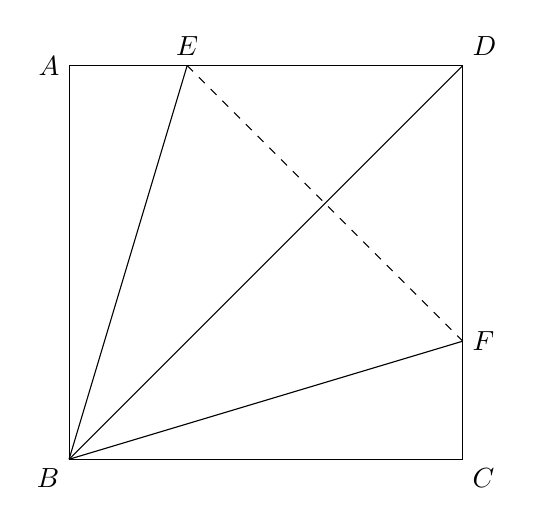
\begin{tikzpicture}
    \coordinate (A) at (0,5);
    \coordinate (B) at (0,0);
    \coordinate (C) at (5,0);
    \coordinate (D) at (5,5);
    \coordinate (E) at (1.5,5);
    \coordinate (F) at (5,1.5);

    % Draw the square outline
    \draw (A) -- (B) -- (C) -- (D) -- (A);

    % Draw solid internal lines
    \draw (B) -- (E);
    \draw (B) -- (D);
    \draw (B) -- (F);

    % Draw dashed line
    \draw[dashed] (E) -- (F);

    % Label points
    \node[left] at (A) {$A$};
    \node[below left] at (B) {$B$};
    \node[below right] at (C) {$C$};
    \node[above right] at (D) {$D$};
    \node[above] at (E) {$E$};
    \node[right] at (F) {$F$};
\end{tikzpicture}
\end{document}
